
In the left menu {\sl Modules$>$Geometry$>$Elementary entities$>$Add} 
choose {\sl Rectangle} and input the coordinates 
of the lower left corner and its size.
Then click on {\sl Tools$>$Options} and {\sl Tools$>$Statistics}. Your screen should look like this:

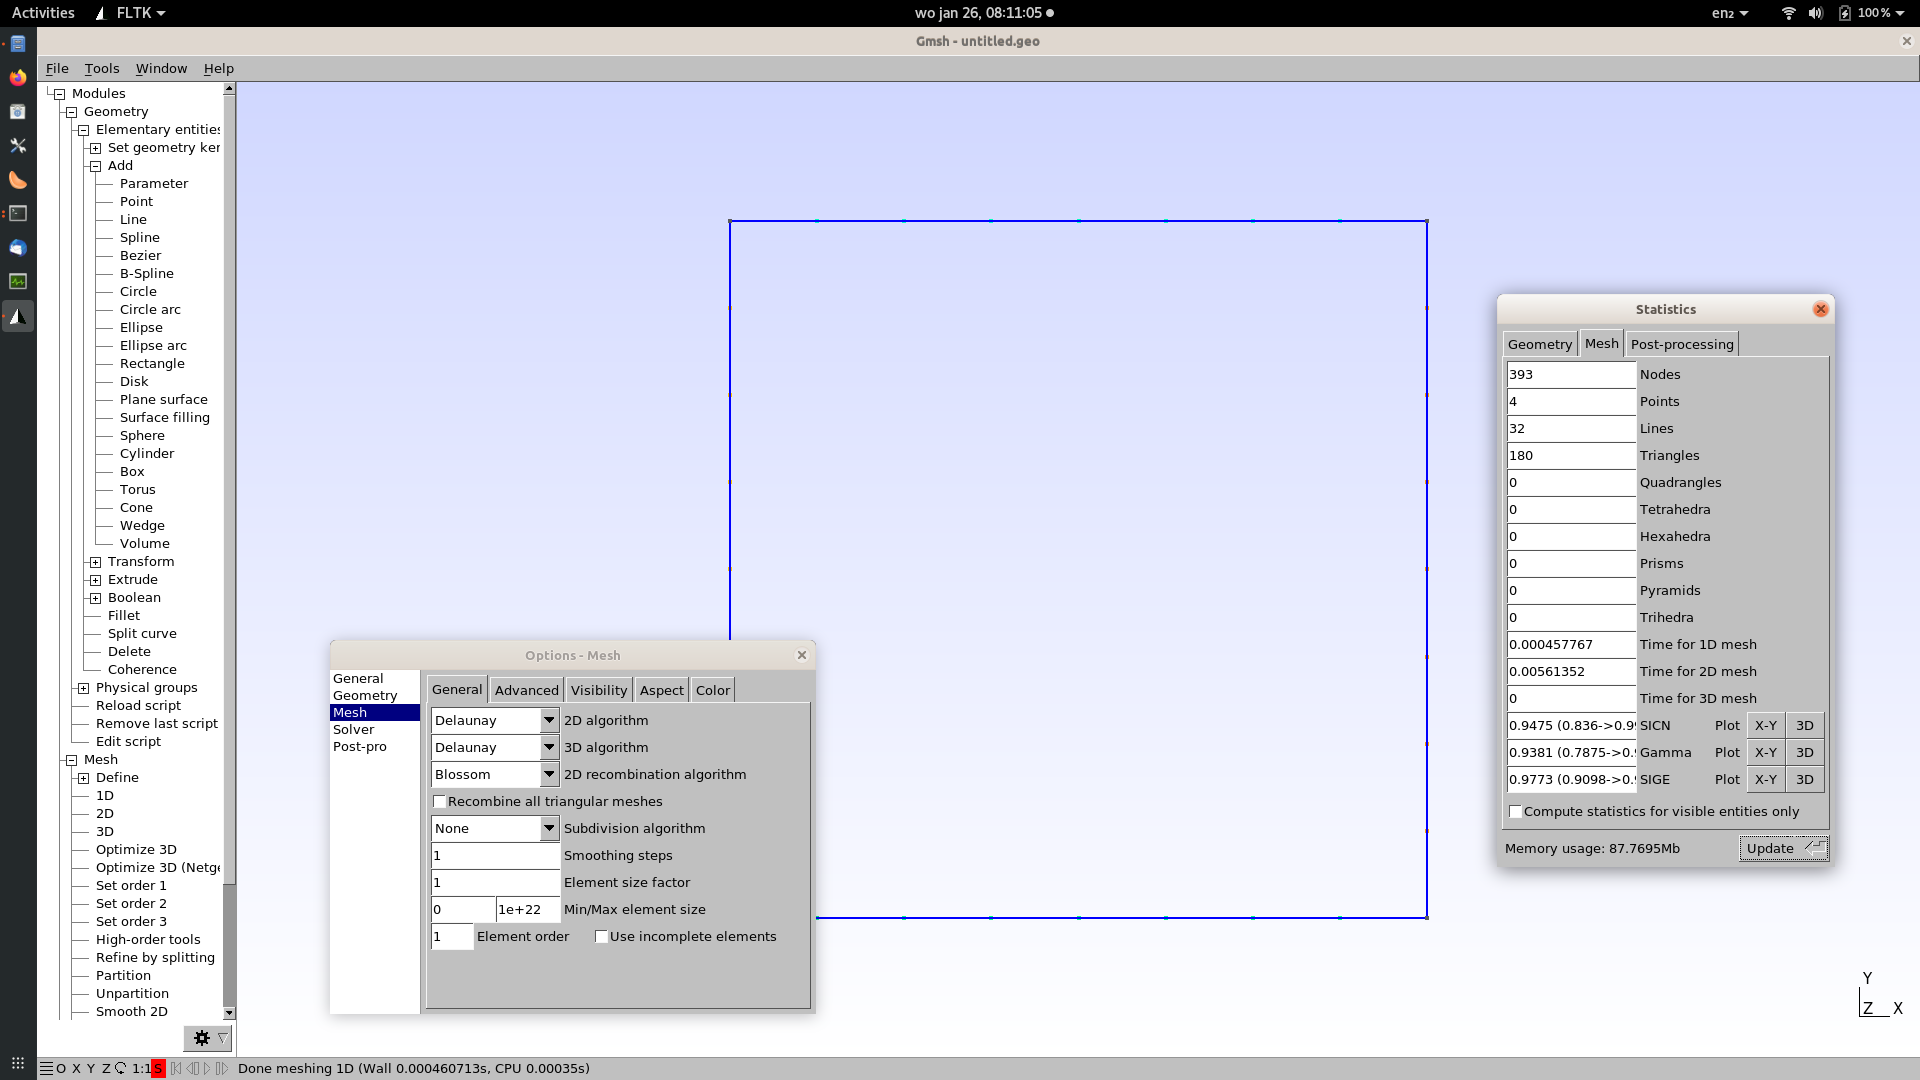
\includegraphics[width=15cm]{images/app_gmsh/gmsh_00}

In the left menu click on {\sl Mesh$>$2D} to generate an unstructured mesh. You should get this:

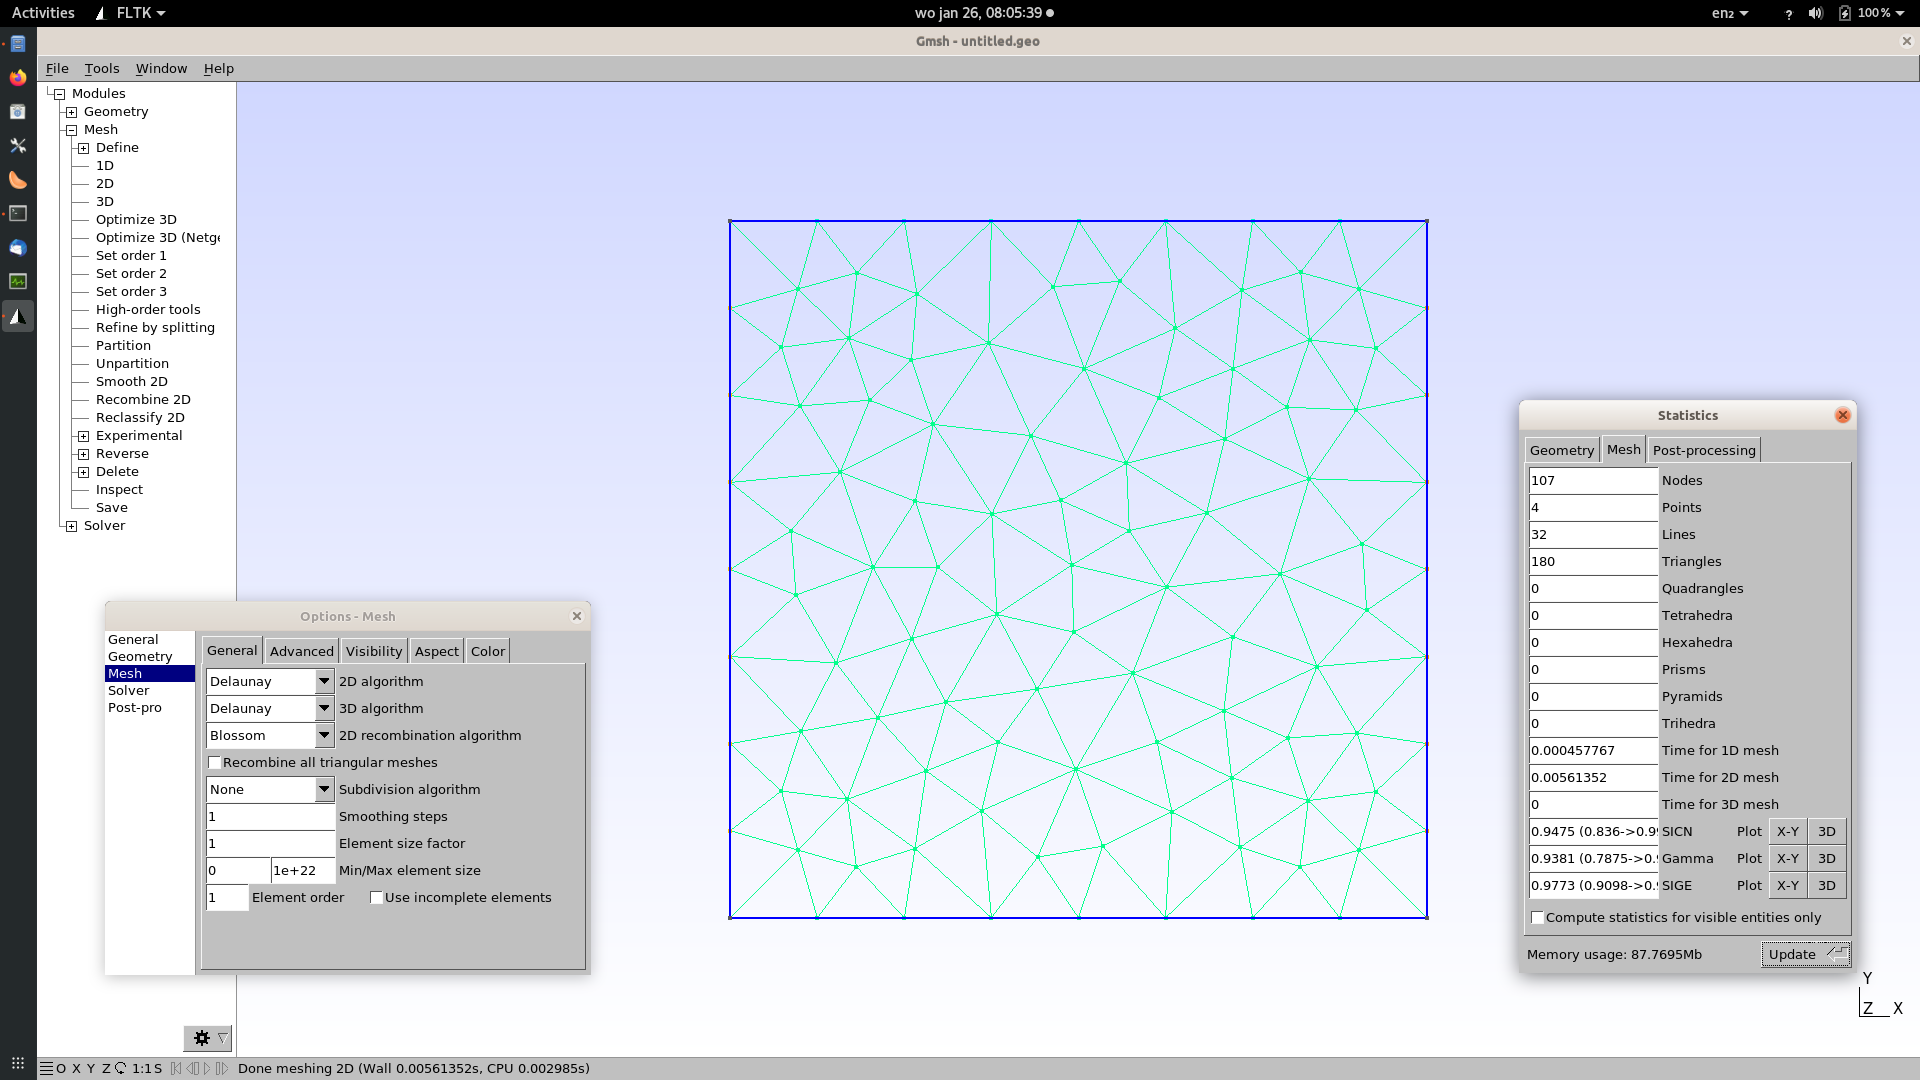
\includegraphics[width=15cm]{images/app_gmsh/gmsh_03}

Make sure you can visualise the nodes by setting:

\begin{center}
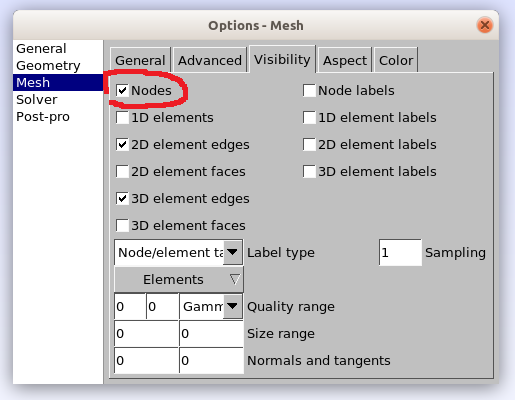
\includegraphics[width=5cm]{images/app_gmsh/gmsh_01}
\end{center}

If you wish to use quadrilaterals

\begin{center}
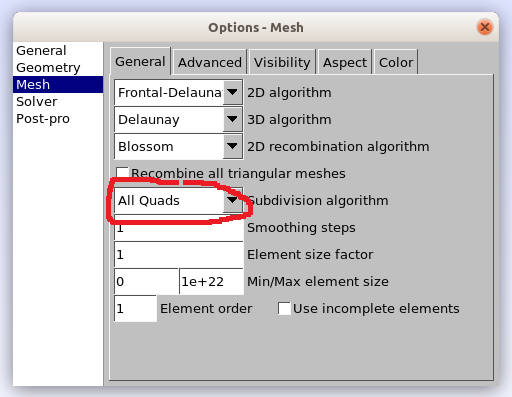
\includegraphics[width=5cm]{images/app_gmsh/gmsh_02}
\end{center}

If you wish to generate second order elements click on {\sl Mesh$>$Set order 2}:

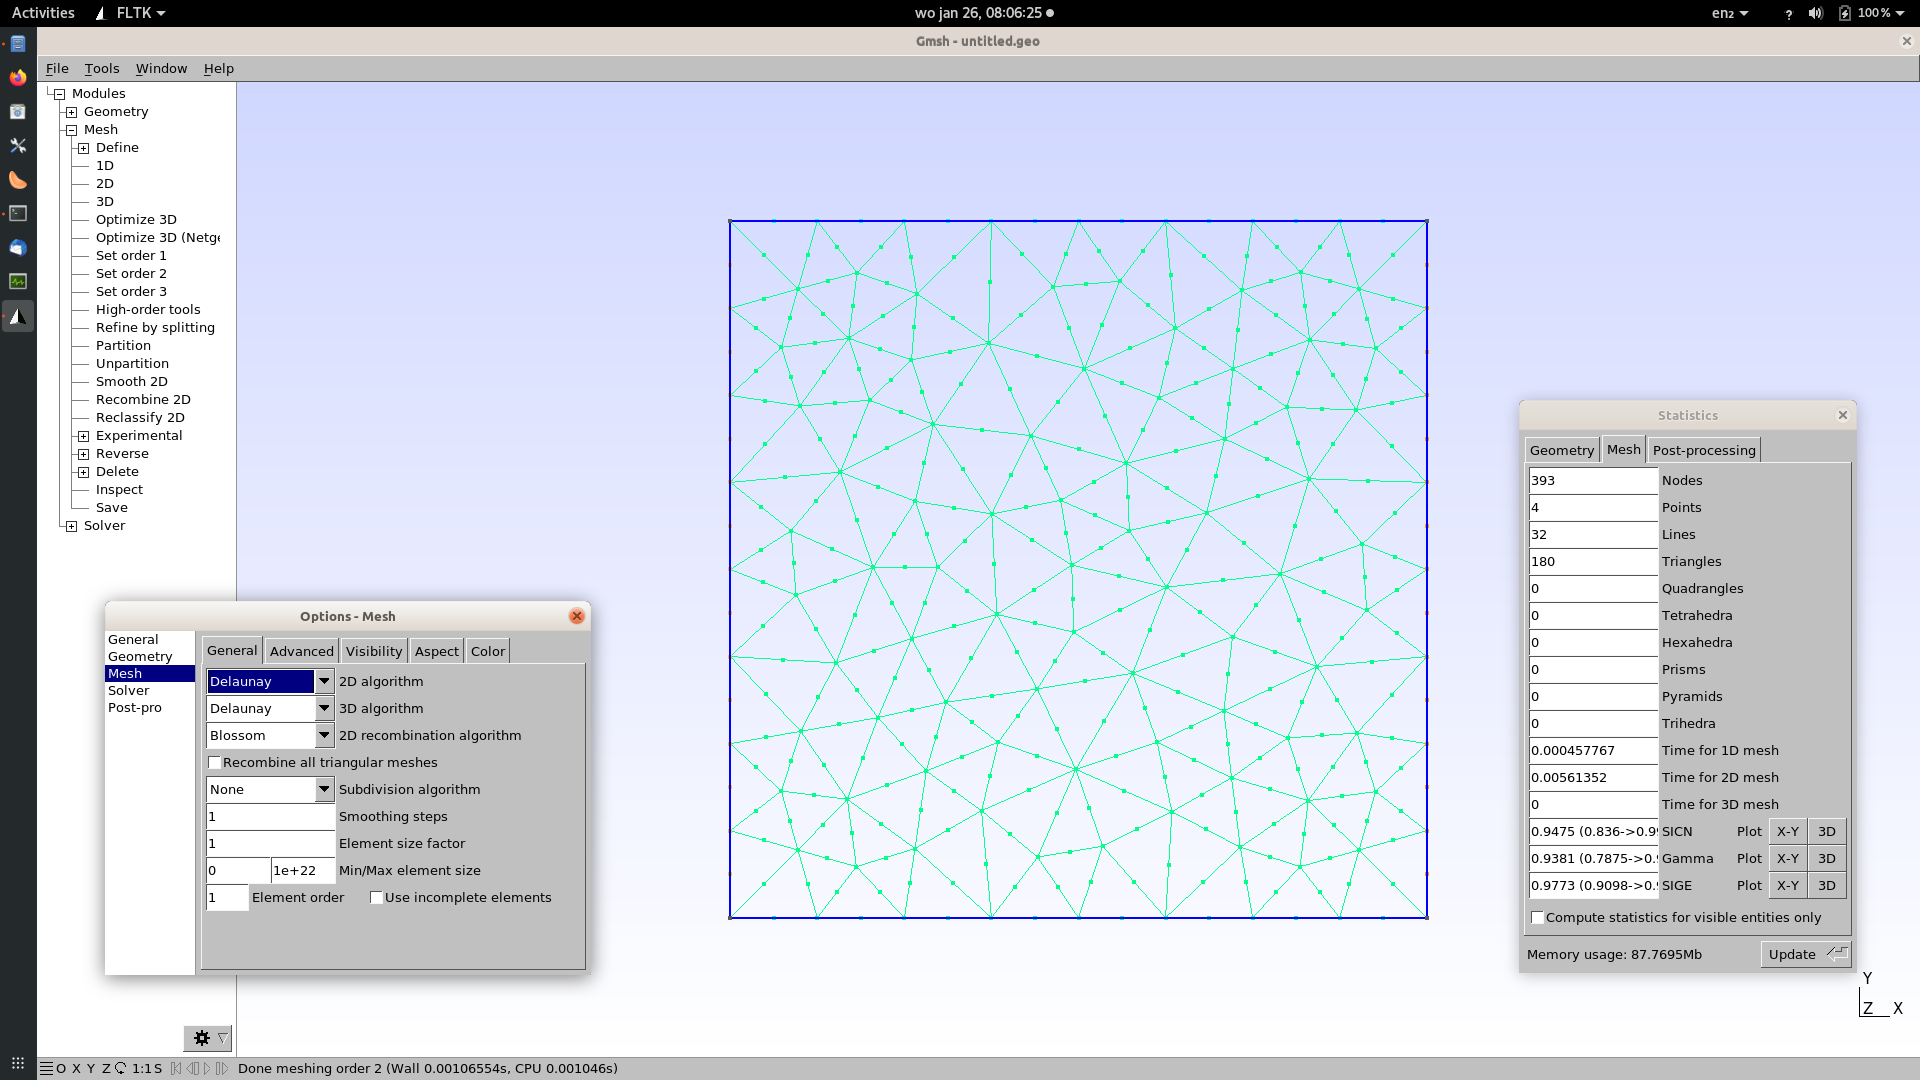
\includegraphics[width=15cm]{images/app_gmsh/gmsh_04}

You can refine the mesh by clicking on {\sl Refine by splitting}

Export the mesh: {\sl File$>$Export}. Choose .mesh format. 

In {\sl Options - General - General tab} click on {\sl Use dark interface} 
and in {\sl Options - Mesh - Visibility tab} click on {\sl Node labels}. Your screen now 
looks like this:

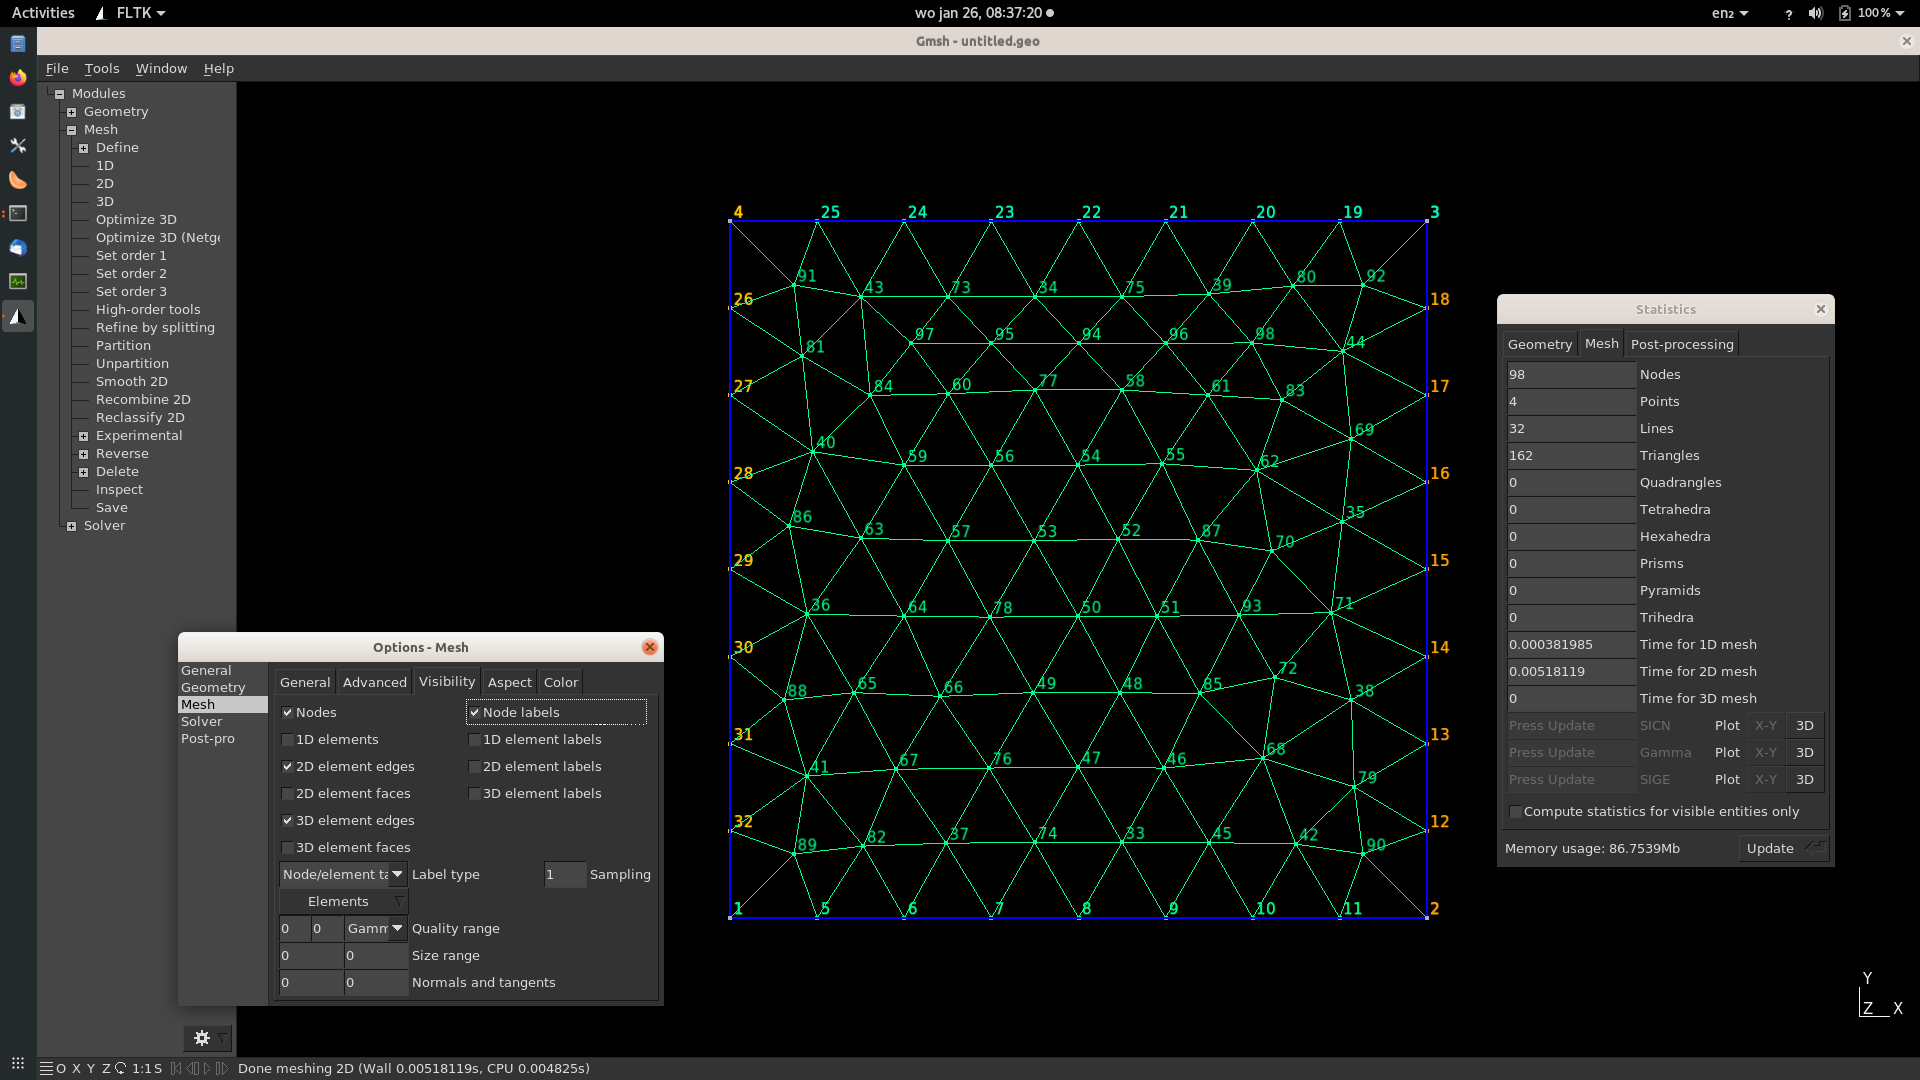
\includegraphics[width=15cm]{images/app_gmsh/gmsh_05}

Also in Options - Mesh - General choose Delaunay instead of Frontal Delaunay to get this 

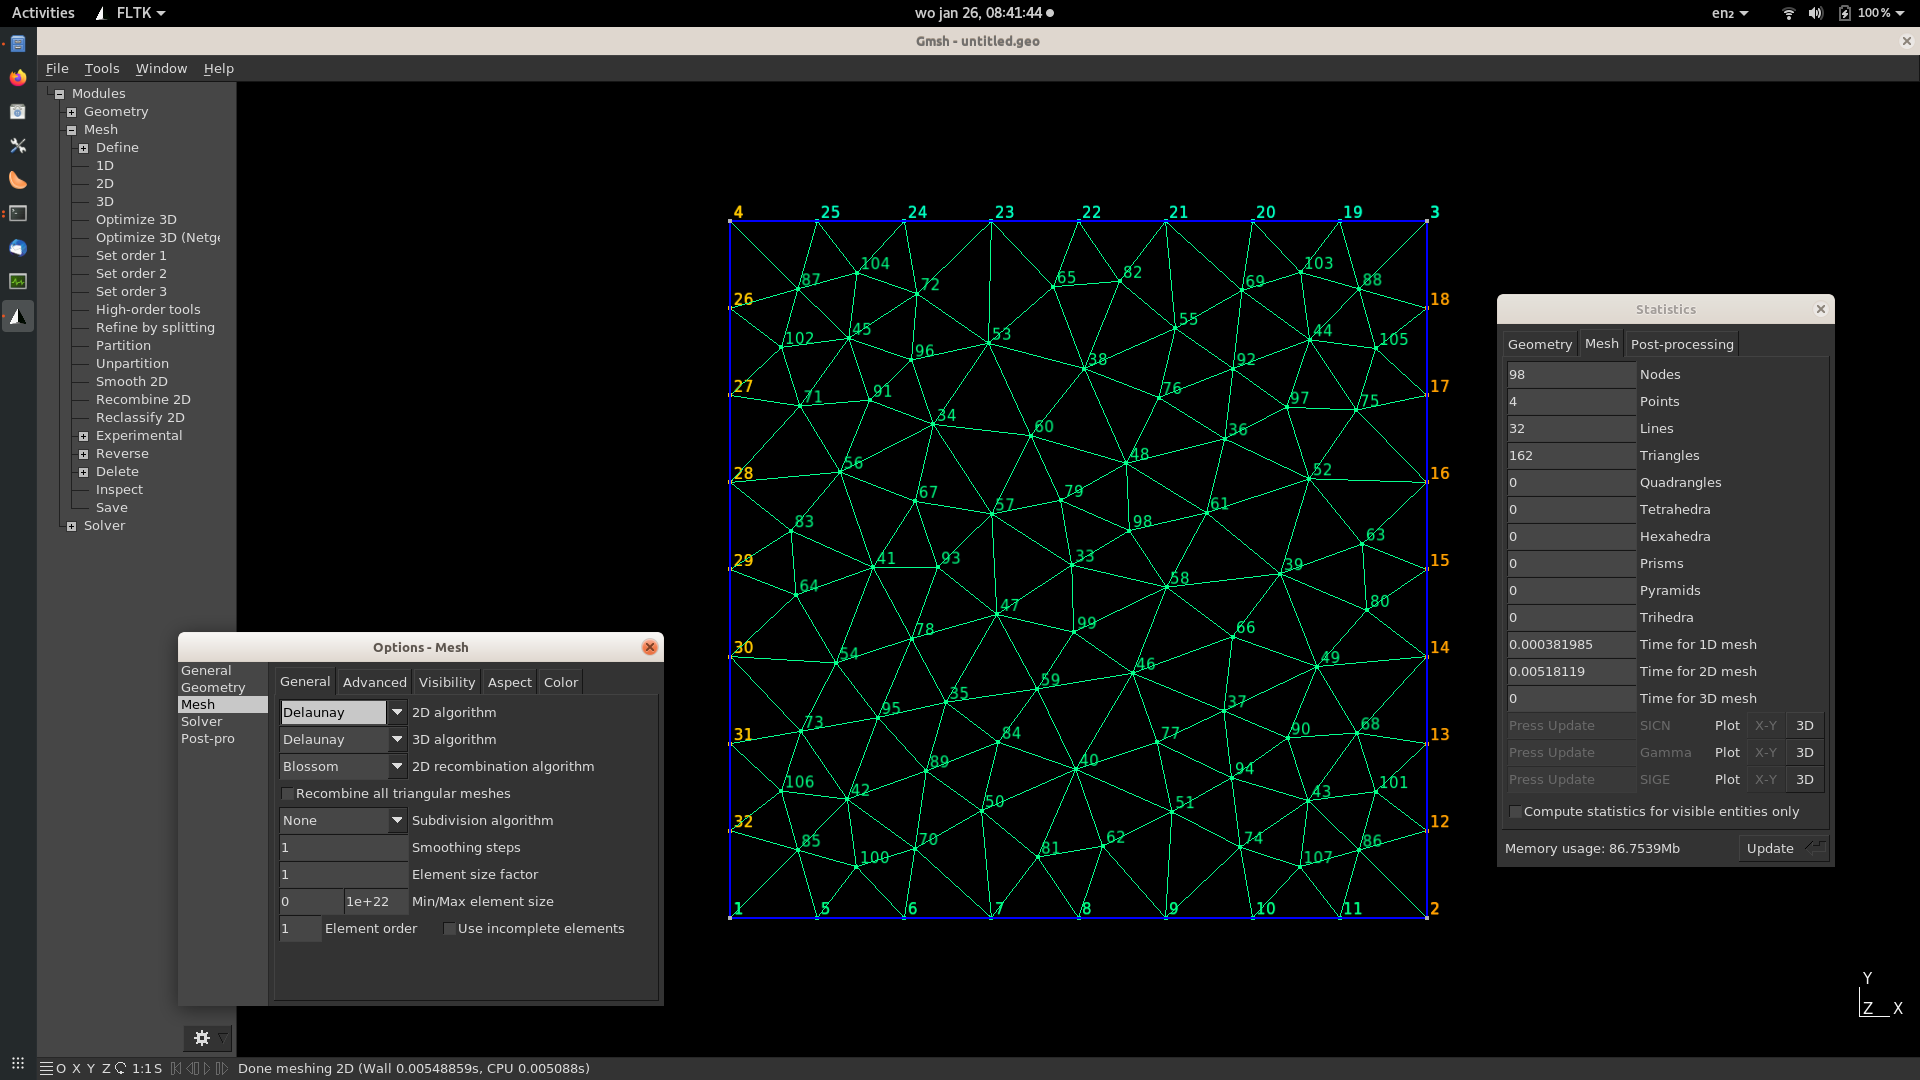
\includegraphics[width=15cm]{images/app_gmsh/gmsh_06}

In order to re-generate a mesh, you mish wish to click on 1D and then on 2D again. 


